\documentclass{beamer} 
\usepackage{graphicx}
\usepackage{url}
\usepackage{fancyvrb}
\usepackage{relsize}
\usepackage{listings}

\lstset{language=R}

\mode<presentation>
{ \usetheme{Hannover} }

\title{Image Fraud Research: Block Artifact Grid Localization} 
\author{Robin Yancey\\
%Advised by Norm Matloff\\
%University of California at Davis \\
%Dept. of Computer Science
}

%\date{Joint Statistical Meetings 2018\\
%Vancouver, Canada
%}
\begin{document} 

 \lstset{language=R}
\lstset{language=R,basicstyle=\smaller,commentstyle=\rmfamily\smaller,
   showstringspaces=false,
   xleftmargin=4ex,literate={<-}{{$\leftarrow$}}1 {~}{{$\sim$}}1}

\begin{frame}
\titlepage

% URL for these slides (repeated on final slide):
% \url{http://heather.cs.ucdavis.edu/parmatpows/Slides.pdf}

\end{frame}


\begin{frame}{What is Block Artifact Grid Localization}

- Block Artifact Grid localization uses the difference in the JPEG compression rates in image blocks to estimate the locations with a high amount of artifacts which are located in the specific blocks in point of forgery 
\newline
-This method is based on the JPEG compression technique (see https://en.wikipedia.org/wiki/JPEG)

\end{frame}




\begin{frame}{Steps 1}



\begin{itemize}

 \item divide the image into 8x8 blocks (as used in JPEG compression)

\item take the DCT of the blocks (using an 8x8 DCT matrix and matrix multiply as done in JPEG compression) 



\textbf{\small{$  im[i:endw,j:endh] <- round(T * im_block * t(T))t  $}}
\newline
* matrix multiply


\end{itemize}

\end{frame}

\begin{frame}{Steps 2}
\begin{itemize}

\item make a histogram of the (quantized between --257 to 257) DCT values for each of the 64 locations of 8x8 blocks (the number of blocks is equal to the number that can fit into the image (eg. round(nrow/8)*round(ncol/8)/ (8x8)) so the number of values in each histogram is equal to the number of blocks
%
\newline
\newline
\textbf{\small{$  hists[i,j,] <- histc(blockdct[i,j,],-257:257)cnt  $}}
%
%

\end{itemize}
\end{frame}


\begin{frame}{Steps 2}
%\titlepage
If the histogram of DCT coefficients
contains periodic patterns, then the coefficients are
likely to have been quantized with a step of this periodic:


\includegraphics[scale=0.4]{/Users/robinyancey/desktop/example_histograms}
\end{frame}






\begin{frame}{Steps 3}



\begin{itemize}

\item take the FFT of the histogram of each of the 64 frequencies to get the periodicity and then power spectrum (absolute value) to get peaks (total size)
\newline
\newline
\textbf{\small{$ onehist <- array(hists[row,col,],c(1,dim(hists)[3]))  $}}
    
\textbf{\small{$     ffthists <- abs(fft(onehist))  $}}

\end{itemize}

\end{frame}


\begin{frame}{Steps 3}
%\titlepage

The power spectrum contains strong peaks (unlike the power spectrum of uncompressed image)

\includegraphics[scale=0.4]{/Users/robinyancey/desktop/powerSpectrum}

\end{frame}

\begin{frame}{Steps 4}


\begin{itemize}


\item calculate the number of local minimums of the filtered second derivative
\textbf{\small{$ secondDiff <- diff(diff(ffthists)) $}}

\item As shown (on the next slide) the local minimum number of peaks plus one is the estimated Q

\end{itemize}

\end{frame}





\begin{frame}{Steps 4}
%\titlepage

The low pass filtered 2nd order derivative (with positive values eliminated) in power spectrum provides a clear view of the peaks:

\includegraphics[scale=0.4]{/Users/robinyancey/desktop/2ndorderDiff}
\end{frame}

\begin{frame}{Steps 5}


\begin{itemize}


\item Once we get a Q estimate for at least 32 Q values in the matrix, we use the estimated Q to calculate the block artifact for each image block:

\textbf{\small{$ imblocks <- abs( blockdct - (Q2*round(blockdct/Q2)) ) $}}
\end{itemize}
\end{frame}

\begin{frame}{Steps 5}
%\titlepage
Here is an image where we can see the cat was forged:
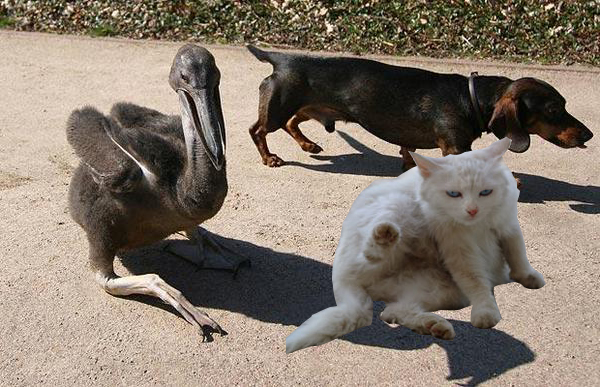
\includegraphics[scale=0.35]{/Users/robinyancey/desktop/Tp_D_NNN_M_N_ani10132_ani10123_12477.jpg}
\end{frame}

\begin{frame}{Steps 5}
%\titlepage
Here is the output showing the heat map over the image. Blocks with a high artifact value from the equation above are bright yellow or red:
\newline
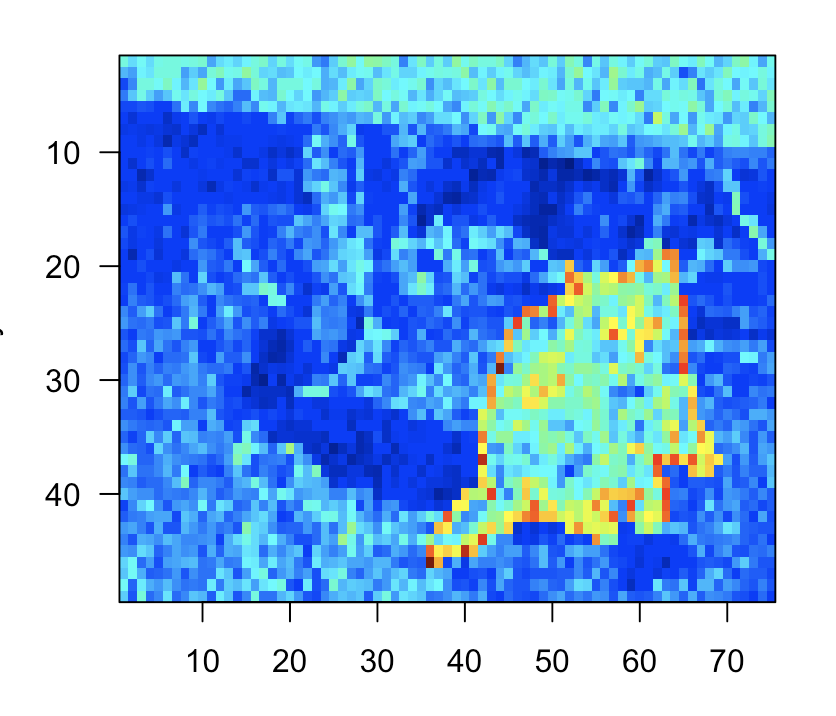
\includegraphics[scale=0.4]{/Users/robinyancey/desktop/Tp_D_NNN_M_N_ani10132_ani10123_12477_OUTPUT}
\end{frame}



%%% new im
\begin{frame}{Steps 5}
%\titlepage
Here is another image where we can see the cat was forged:
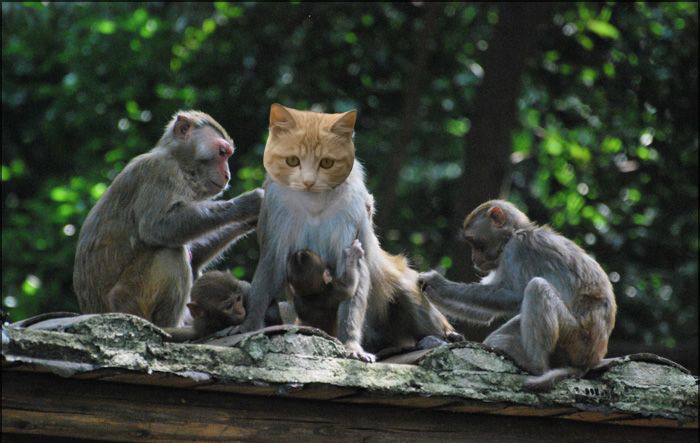
\includegraphics[scale=0.35]{/Users/robinyancey/desktop/Tp_D_NRN_S_N_ani10210_ani10209_12373.jpg}
\end{frame}

\begin{frame}{Steps 5}
%\titlepage
Here is another example output:
\newline
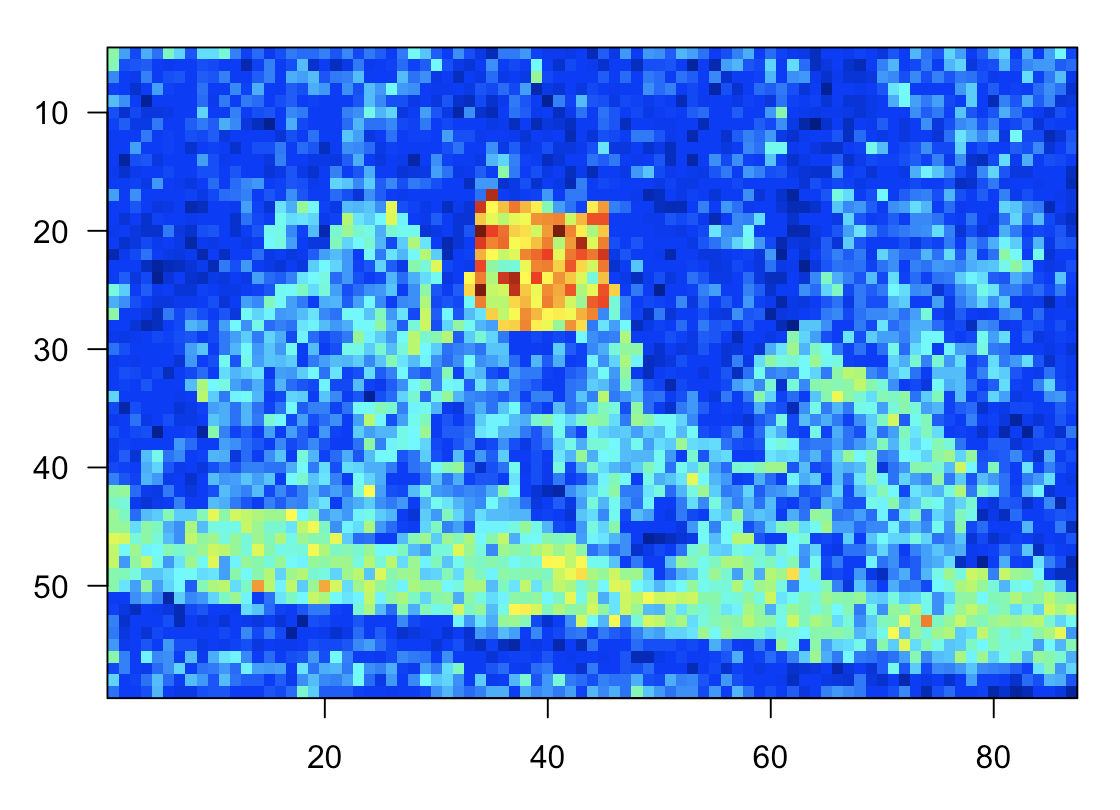
\includegraphics[scale=0.4]{/Users/robinyancey/desktop/Tp_D_NRN_S_N_ani10210_ani10209_12373_OUTPUT}
\end{frame}


\end{document}
